%!TEX program = xelatex
\documentclass[a4papers]{ctexart}
%数学符号
\usepackage{amssymb}
\usepackage{amsmath}
%表格
\usepackage{graphicx,floatrow}
\usepackage{array}
\usepackage{booktabs}
\usepackage{makecell}
%页边距
\usepackage{geometry}
\geometry{left=2cm,right=2cm,top=2cm,bottom=2cm}

%首行缩进两字符 利用\indent \noindent进行控制
\usepackage{indentfirst}
\setlength{\parindent}{2em}

\setromanfont{Songti SC}
%\setromanfont{Heiti SC}

\usepackage{pstricks,pst-plot}


\title{STATS100B--Introduction to Mathematical Statistics \\Homework 5}
\author{Feng Shiwei \ UID:305256428}
\date{}
\begin{document}
\maketitle
\section*{Exercise a}
\noindent(1) Solution:
\indent 
\[ X\sim F_{m,n},\, Y=\dfrac{1}{X}\sim F_{n,m}  \]
\[ P(X<F_{\alpha;m,n}) = \alpha\]
\[ P(\dfrac{1}{X} > \dfrac{1}{F_{\alpha;m,n}}) = \alpha\]
\[ P(Y > \dfrac{1}{F_{\alpha;m,n}}) = 1-\alpha\]
\[ P(Y < \dfrac{1}{F_{\alpha;m,n}}) = \alpha\]
\[ \therefore \dfrac{1}{F_{\alpha;m,n}} = F_{1-\alpha;n,m},\, \]
    which means
\[ F_{\alpha;m,n} = \dfrac{1}{F_{1-\alpha;n,m}} \]
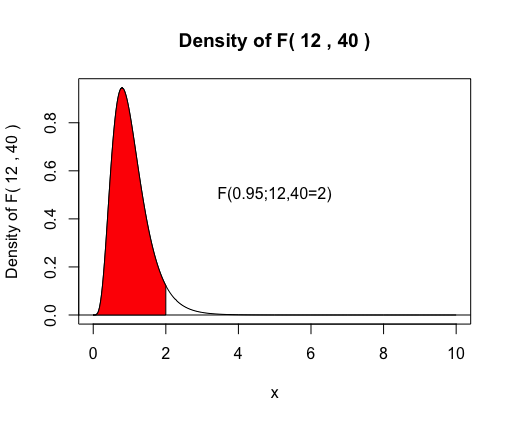
\includegraphics[width=3.5in, height=2.8in]{f-12-40.png}
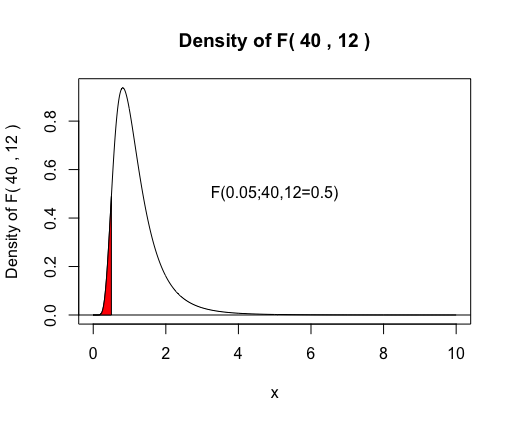
\includegraphics[width=3.5in, height=2.8in]{f-40-12.png}

\noindent (2) Solution:
\[ Y\sim t_n,\, X=Y^2\sim F_{1,n} \]
\[ P(-t_{1-\frac{\alpha}{2},n}<Y<t_{1-\frac{\alpha}{2},n}) = 1-\alpha \]
\[ P(Y^2 < t^2_{1-\frac{\alpha}{2},n}) = 1-\alpha \]
\[ P(X < t^2_{1-\frac{\alpha}{2},n}) = 1-\alpha \]
\[ \therefore t^2_{1-\frac{\alpha}{2},n} = F_{1-\alpha;1,n}\]
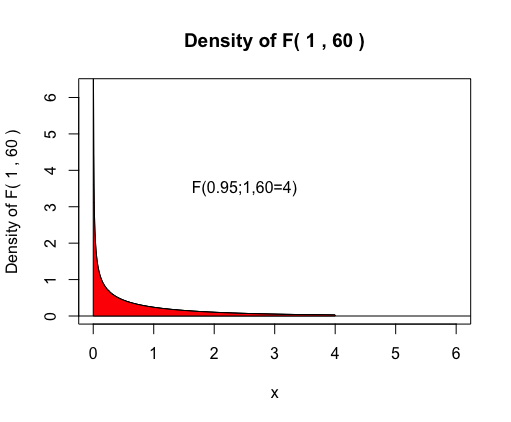
\includegraphics[width=3.5in, height=2.8in]{f-1-60.png}
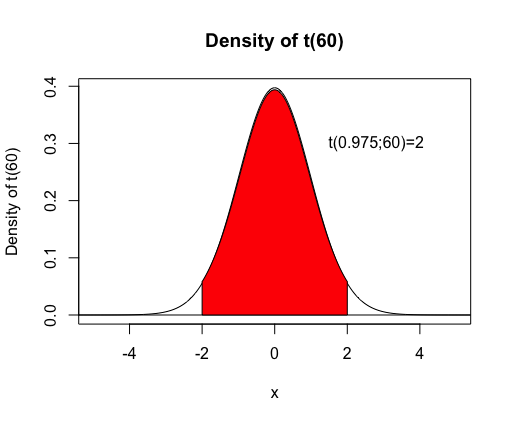
\includegraphics[width=3.5in, height=2.8in]{t-60.png}

\section*{Exercise b}
\noindent Solution:\\
\[ \because \bar{X} \sim N(\mu_1,\dfrac{\sigma_1}{\sqrt{13}}),\,
   \bar{Y} \sim N(\mu_2,\dfrac{\sigma_2}{\sqrt{16}})\]
\[ \therefore \overline {X}+\overline {Y}\sim N\left( \mu _{1}+\mu _{2},\sqrt {\dfrac {\sigma ^{2}_{1}}{13}+\dfrac {\sigma ^{2}_{2}}{16}}\right) \]
\[ \dfrac {\left( \overline {X}+\overline {Y}\right) -\left( \mu _{1}+\mu _{2}\right) }{\sqrt {\dfrac {\sigma ^{2}_{1}}{13}+\dfrac {\sigma ^{2}_{2}}{16}}}\sim N\left( 0,1\right) \]
\[ \because \dfrac{12 S_X^{2}}{\sigma_1}\sim \chi^2_{12},\,
    \dfrac{15 S_Y^{2}}{\sigma_2}\sim \chi^2_{15}\]
\[  \dfrac{12 S_X^{2}}{\sigma_1} + \dfrac{15 S_Y^{2}}{\sigma_2} \sim \chi^2_{27}\]
\[ \therefore \dfrac{ \dfrac {\left( \overline {X}+\overline {Y}\right) -\left( \mu _{1}+\mu _{2}\right) }{\sqrt {\frac {\sigma ^{2}_{1}}{13}+\frac {\sigma ^{2}_{2}}{16}}}}{ \sqrt{\dfrac{\frac{12 S_X^{2}}{\sigma_1} + \frac{15 S_Y^{2}}{\sigma_2}}{27}}} \sim t_{27} \]


\section*{Exercise c}
\noindent Solution:\
\[  \]
\begin{alignat*}{2}
    E(X) 
    &= E\left[\dfrac{\chi^2_{n}/n}{\chi^2_{m}/m}\right] \\
    &= \dfrac{m}{n}E\left[\chi^2_{n} \right] E\left[ (\chi^2_{m})^{-1} \right] \\
    &= \dfrac{m}{n}\cdot n\cdot \dfrac{\Gamma(\dfrac{m}{2}-1)\cdot 2^{-1} }{\Gamma(\dfrac{m}{2})} \\
    &= m \cdot \dfrac{1}{2(\dfrac{m}{2}-1)}\\
    &= \dfrac{m}{m-2}
\end{alignat*}
\begin{alignat*}{2}
    var(X)
    &= var\left[\dfrac{\chi^2_{n}/n}{\chi^2_{m}/m} \right]\\
    &= E\left[\left(\dfrac{\chi^2_{n}/n}{\chi^2_{m}/m}\right)^2\right]-\Bigg(E\left(\dfrac{\chi^2_{n}/n}{\chi^2_{m}/m} \right)\Bigg)^2\\
    &=\dfrac{m^2}{n^2} \cdot E\Big[(\chi^2_n)^2\Big] \cdot E\Big[(\chi^2_m)^{-2} \Big]
        - \dfrac{m^2}{n^2}\cdot \Big(E(\chi^2_n) \Big)^2 \cdot \Big(E\left[(\chi^2_m)^{-1}\right] \Big)^2\\
    &=\dfrac{m^2}{n^2} \times \dfrac{\Gamma(\dfrac{n}{2}+2)\cdot 2^{2} }{\Gamma(\dfrac{n}{2})} \times \dfrac{\Gamma(\dfrac{m}{2}-2)\cdot 2^{-2} }{\Gamma(\dfrac{m}{2})} 
        - \dfrac{m^2}{n^2}\times n^2 \times \Big( \dfrac{\Gamma(\dfrac{m}{2}-1)\cdot 2^{-1} }{\Gamma(\dfrac{m}{2})}  \Big)^2\\
    &= \dfrac{m^2}{n^2} \times n(n+2) \times \dfrac{1}{(m-2)(m-4)}
        - \dfrac{m^2}{n^2} \times n^2 \times \dfrac{1}{(m-2)^2}\\
    &= \dfrac{2m^2(m+n-2)}{n(m-2)^2(m-4)}
\end{alignat*}


\section*{Exercise d}
\[  \bar{X}=\dfrac{1}{n}\boldsymbol{1}'\boldsymbol{X},\, \boldsymbol{1}=(1\, 1\, \cdots 1)'\]
\[  \begin{pmatrix} \bar{X}\\ X_1-\bar{X}\\X_2-\bar{X}\\ \cdots \\ X_n-\bar{X} \end{pmatrix}
    = \begin{pmatrix}
        \dfrac{1}{n}\boldsymbol{1}' \\ \boldsymbol{I}-\dfrac{1}{n}\boldsymbol{1}\boldsymbol{1}'
    \end{pmatrix}
    = \boldsymbol{A}\boldsymbol{X}
    \]
\begin{alignat*}{2}
    var(\boldsymbol{A}\boldsymbol{X})  
    &=  \begin{pmatrix}\dfrac{1}{n}\boldsymbol{1}' \\ \boldsymbol{I}-\dfrac{1}{n}\boldsymbol{1}\boldsymbol{1}' \end{pmatrix} 
        \begin{pmatrix} (1-\rho)\boldsymbol{I}-\rho\boldsymbol{J}\end{pmatrix}
       \begin{pmatrix}\dfrac{1}{n}\boldsymbol{1}' & \boldsymbol{I}-\dfrac{1}{n}\boldsymbol{1}\boldsymbol{1}' \end{pmatrix} 
\end{alignat*}
Notice that\[ \boldsymbol{1}'\boldsymbol{1}=n,\,\boldsymbol{1}\boldsymbol{1}'=\boldsymbol{J},\,
             \boldsymbol{1}'\boldsymbol{J}=n\boldsymbol{1}',\,\boldsymbol{J}\boldsymbol{1}=n\boldsymbol{1}\]

\[\therefore
    var(\boldsymbol{A}\boldsymbol{X})=\begin{pmatrix}
        (1-\rho)\dfrac{1}{n}+\rho & \boldsymbol{0}\\
        \boldsymbol{0} & (1-\rho)(\boldsymbol{I}-\dfrac{1}{n}\boldsymbol{1}\boldsymbol{1}')
    \end{pmatrix} \]    
\[ \therefore \bar{X}\,  and\,\begin{pmatrix}  X_1-\bar{X}\\X_2-\bar{X}\\ \cdots \\ X_n-\bar{X} \end{pmatrix}\, are \,\,  independent. \]         


\section*{Exercise e}
\begin{alignat*}{2}
    \boldsymbol{Y}' \boldsymbol{\Sigma}\boldsymbol{Y} 
    &=\begin{pmatrix}Y_1 \\ Y_2 \end{pmatrix} \dfrac{1}{\sigma_1^2\sigma_2^2-\sigma_{12}^2}
        \begin{pmatrix}\sigma_2^2 & -\sigma_{12} \\ -\sigma_{21} & \sigma_1^2 \end{pmatrix}
        \begin{pmatrix}Y_1 & Y_2 \end{pmatrix} \\
    &= \dfrac {\sigma ^{2}_{2}Y^{2}_{1}-2\sigma _{12}Y_{1}Y_{2}+\sigma ^{2}_{1}Y^{2}_{2}}{\sigma ^{2}_{1}\sigma ^{2}_{2}-\sigma ^{2}_{12}}
    \end{alignat*}

\begin{alignat*}{2}
    \boldsymbol{Y}' \boldsymbol{\Sigma}\boldsymbol{Y} -\dfrac{Y_1^2}{\sigma_1^2}
    &= \dfrac {\sigma ^{2}_{2}Y^{2}_{1}-2\sigma _{12}Y_{1}Y_{2}+\sigma ^{2}_{1}Y^{2}_{2}-\sigma ^{2}_{1}\sigma ^{2}_{2}\left( 1-\rho ^{2}\right) \dfrac {Y^{2}_{1}}{\sigma ^{2}_{1}}}{\sigma ^{2}_{1}\sigma ^{2}_{2}\left( 1-\rho ^{2}\right) }\\
    &= \dfrac {\dfrac {Y^{2}_{1}}{\sigma ^{2}_{1}}-2\rho \dfrac {y_{1}}{\sigma _{1}}\dfrac {Y_{2}}{\sigma _{2}}+\dfrac {Y^{2}_{2}}{\sigma ^{2}_{2}}-\left( 1-\rho ^{2}\right) \dfrac {Y^{2}_{1}}{\sigma ^{2}_{1}}}{1-\rho }\\
    &= \dfrac {\left( \rho \dfrac {Y_{1}}{\sigma _{1}}-\dfrac {Y_{2}}{\sigma _{2}}\right) ^{2}}{1-\rho ^{2}}
\end{alignat*}

\[ \because
    \begin{pmatrix} \rho \dfrac {Y_{1}}{\sigma _{1}} & -\dfrac {Y_{2}}{\sigma _{2}} \end{pmatrix}
    = \begin{pmatrix} \dfrac{\rho}{\sigma_1} & -\dfrac{1}{\sigma_2} \end{pmatrix}
      \begin{pmatrix} Y_1 \\ Y_2  \end{pmatrix}
\]

\begin{alignat*}{2}
    var\Bigg( \begin{pmatrix} \rho \dfrac {Y_{1}}{\sigma _{1}} & -\dfrac {Y_{2}}{\sigma _{2}} \end{pmatrix} \Bigg) 
    &= \begin{pmatrix} \dfrac{\rho}{\sigma_1} & -\dfrac{1}{\sigma_2} \end{pmatrix} 
       \begin{pmatrix}\sigma_2^2 & -\sigma_{12} \\ -\sigma_{21} & \sigma_1^2 \end{pmatrix}
       \begin{pmatrix} \frac{\rho}{\sigma_1} \\ -\frac{1}{\sigma_2} \end{pmatrix} 
    &= 1-\rho^2
\end{alignat*}
\[  
    E\Bigg(
            \begin{pmatrix} \rho \dfrac {Y_{1}}{\sigma _{1}} & -\dfrac {Y_{2}}{\sigma _{2}} \end{pmatrix}
    \Bigg) 
    = \dfrac {\rho}{\sigma _{1}}\times 0 -\dfrac {1}{\sigma _{2}}\times 0 = 0
\]
\[ \therefore \dfrac{ \rho \dfrac {Y_{1}}{\sigma _{1}}-\dfrac {Y_{2}}{\sigma _{2}}}{\sqrt{1-\rho^2}} \sim N(0,1) \]
\[ \boldsymbol{Y}' \boldsymbol{\Sigma}\boldsymbol{Y} - \dfrac{Y_1^2}{\sigma_1^2}
    = \dfrac {\left( \rho \dfrac {Y_{1}}{\sigma _{1}}-\dfrac {Y_{2}}{\sigma _{2}}\right) ^{2}}{1-\rho ^{2}} \sim \chi^2_1
\]


    
\end{document}